\begin{frame}{Fundamentação Teórica}
    As seções posteriores, agruparão os conceitos em elementos: Base do projeto, \textit{Hardware}, \textit{Firmware} e \textit{Software}.  
\end{frame}

\begin{frame}{Elementos Base}{Redes \textit{Wireless}}
      
\begin{itemize}
    \item O termo \textit{Wireless} provém do inglês: \textit{wire} (fio, cabo); less (sem);
    \medskip
    \item Possui vantagens cruciais para a aplicação do conceito de Internet das Coisas:
\end{itemize}    

\end{frame}

\begin{frame}{Elementos Base}{Redes \textit{Wireless}}
      
    \begin{itemize}
        \item \textbf{Maior produtividade - } disponibiliza acesso à rede em todo o raio de alcance onde o ponto de acesso está instalado, oferecendo liberdade de deslocamento com conexão contínua;
	
        \item \textbf{Flexibilidade de instalação -} podem ser instaladas em locais com temperaturas elevadas, em que os cabos não suportariam, ou em locais que necessitam de acesso temporário;
        
        \item \textbf{Redução de custo - } reduzem os custos de instalação, dispensando o uso de material para cada ponto de conexão;
        
        \item \textbf{Interoperabilidade e segurança - } capaz de comunicar sistemas de forma confiável e com segurança, possuindo chaves de acesso e até mesmo transferindo mensagens criptografadas.   
    \end{itemize}    
    
\end{frame}

\begin{frame}{Elementos Base}{Redes \textit{Wireless}}
    A topologia de uma rede IEEE 802.11 (\textit{Wi-Fi})  possui os seguintes elementos-chave:

    \begin{itemize}
        \item \textbf{BSS - \textit{Basic Service Set} -} corresponde a uma célula de comunicação \textit{wireless};
        \item \textbf{STA - \textit{Stations} -} são as estações de trabalho que comunicam-se entre si dendo da \textbf{BSS};
        \item \textbf{AP - \textit{Access Point} -} coordena a comunicação entre as \textbf{STA's} dentro da \textbf{BSS}. Na maioria das vezes roteadores realizam tal operação;
        
    \end{itemize}
    
\end{frame}

\begin{frame}{Elementos Base}{Redes \textit{Wireless}}
    \begin{itemize}
    \item \textbf{\textit{Bridge} -} faz a ligação entre diferentes redes, por exemplo, uma rede sem fio para uma rede cabeada convencional;
	\item  \textbf{ESS - \textit{Estended Service Set} -} consiste de várias células \textbf{BSS's} vizinhas que se interceptam e cujos \textbf{AP's} estão conectados a uma mesma rede tradicional. Nestas condições uma \textbf{STA} pode movimentar-se de um \textbf{BSS} para outr, permanecendo conectada à rede. Este processo é denominado \textit{Roaming}.
	\end{itemize}
\end{frame}

\begin{frame}{Elementos Base}{A Internet das Coisas}
    \begin{itemize}
        \item Um conjunto de tecnologias e protocolos associados que permitem que objetos se conectem a uma rede de comunicações e onde são identificados e controlados;
        \item Esse termo se tornou possível graças aos avanços tecnológicos e as reduções de custo de todos os dispositivos eletroeletrônicos, os quais possuem a capacidade de comunicação principalmente por meio de protocolos \textit{Wiress};
    \end{itemize}
    
\end{frame}

\begin{frame}{Elementos Base}{A Internet das Coisas}

    \begin{figure}
        \centering
        \caption{Protocolos utilizados para aplicacão do \textit{IoT} com base nos conceitos de redes. Relação entre velocidade-força e distância.}
        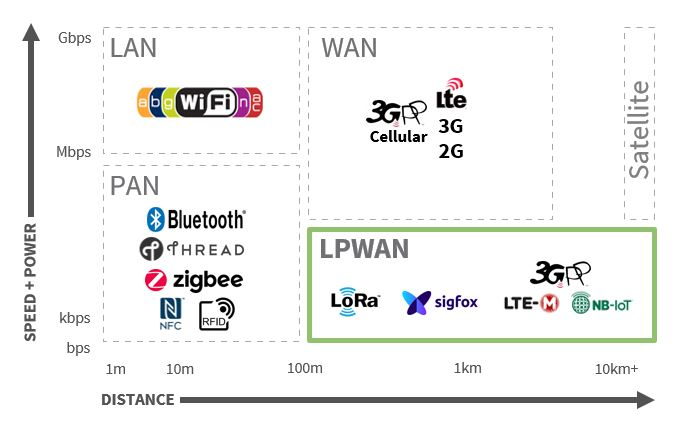
\includegraphics[width=0.6\linewidth]{figuras/iotprotocols.jpg}
        \caption*{\small{Fonte: iot.do, 2021}}
    \end{figure}   

\end{frame}


\begin{frame}{Elementos Base}{O protocolo MQTT}

    \begin{itemize}
        \item \textbf{\textit{Message Queuing Telemetry Transport}} - MQTT foi inventado e desenvolvido inicialmente pela \textit{International Business Machines} - IBM;
        \item É um protocolo de mensagem com suporte para a comunicação \textbf{assíncrona} entre as partes;
        \item Projetado para aplicações que utilizam pouca banda de rede utilizando um modelo de publicação e assinatura;

    \end{itemize}


\end{frame}

\begin{frame}{Elementos Base}{O protocolo MQTT}

    \begin{itemize}
        \item Em uma rede MQTT existem dois agentes principais: o \textit{\textbf{broker}} e os \textit{\textbf{clients}};
        \item O \textit{broker} é um servidor que centraliza as mensagens dos clientes e as encaminha para os clientes interessados;
        \item É um dispositivo ou serviço que tenha capacidade de interagir com o \textit{broker} e trocar mensagens;

    \end{itemize}


\end{frame}

\begin{frame}{Elementos Base}{O protocolo MQTT}

    \begin{figure}[H]
        \centering
        \caption{Diagrama básico MQTT}
        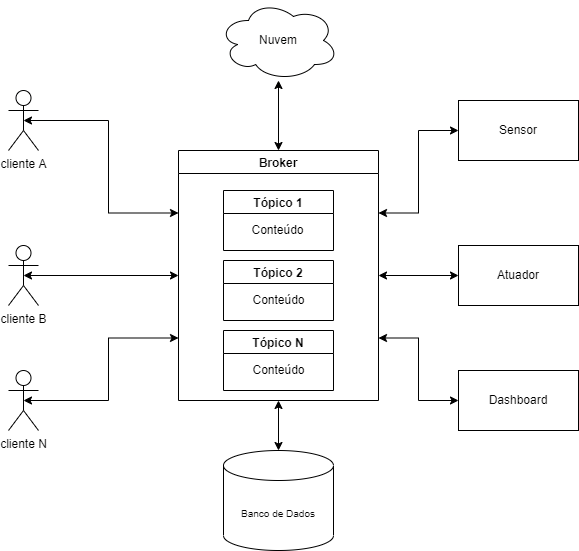
\includegraphics[width=0.45\textwidth]{figuras/mqtt.drawio.png}
        \caption*{\small{Fonte: própria, 2021}}
        \label{fig:mqtt_diagram}
    \end{figure}

\end{frame}

\begin{frame}{Elementos Base}{O protocolo MQTT}
    \begin{itemize}
        \item Como qualquer outro protocolo de comunicação o MQTT possui diversos termos e características associadas, como a segurança, a definição dos \textit{endpoints}\footnote{\textbf{endpoints} - Pontos de extremidade. Terminais de conexão entre uma API e o cliente.}, o endereçamento, tipo de dado trafegado, entre outros.
    \end{itemize}

\end{frame}

\begin{frame}{Elementos Base}{O protocolo MQTT}
    \begin{itemize}
        \item \textbf{\textit{broker}}: É o intermediário no processo de comunicação, atuando como um servidor;
        \item \textbf{\textit{client}}: Responsável por estabelecer e manter uma conexão com o \textit{broker}, enviar e receber as mensagens;
        \item \textit{\textbf{broker ip}}: Identificação única do servidor \textit{\textbf{broker}} conectado em determinada rede;
        \item \textbf{\textit{broker username e broker password}}: Credenciais, opcionais, para determinado cliente estabelecer conexão com o servidor; 
    \end{itemize}

\end{frame}

\begin{frame}{Elementos Base}{O protocolo MQTT}
    \begin{itemize}
        \item  \textit{\textbf{QoS}}: Nível de qualidade do serviço desejado, indicando como deve ser a relação entre os elementos comunicantes.\cite{fabiobrandao};
        \item \textbf{\textit{last good message}}: É a operação à qual o \textit{broker} envia a última menagem válida recebida em um determinado tópico ao ser requisitado por um cliente;
        \item \textbf{\textit{last will testament (LWT)}}: São mensagens pré-definidas a serem publicadas pelo broker em nome de um determinado cliente, uma vez que esse cliente está \textit{offline} e não pode publicar mais;
        \item \textbf{\textit{keep alive}}: Mensagens periódicas enviadas por determinado cliente buscando validar a conexão;
    \end{itemize}

\end{frame}

\begin{frame}{Elementos Base}{O protocolo MQTT}
    \begin{itemize}
        \item \textbf{tópicos, \textit{publish} e \textit{subscribe}}: O ato de um cliente enviar uma mensagem é chamado \textit{publish}(publicação). E para receber mensagens de determinado um tópico um cliente deve fazer um \textit{subscribe}(inscrição). Os níveis de um tópico são separados por “/” e um cliente pode optar por se inscrever em quantos tópicos forem necessários, utilizando os artifícios da \autoref{tab:simbolos_mqtt}.
    \end{itemize}

\end{frame}

\begin{frame}{Elementos Base}{O protocolo MQTT}
    \begin{table}[H]
        \centering
        \resizebox{\textwidth}{!}{%
            \begin{tabular}{c|c|c}
                \hline
                Símbolos & Descrição & Exemplo \\ \hline
                + & Retorna ou envia qualquer informação naquele nível (Coringa) & \begin{tabular}[c]{@{}c@{}}area/10/sensor/5000/temperatura\\ area/10/sensor/4000/temperatura\\ area/10/sensor/+/temperatura\end{tabular} \\ \hline
                \# & Retorna ou envia qualquer coisa abaixo daquele nível & area/10/\# \\ \hline
                \$ & Tópicos iniciados com \$ são especiais usados internamente pelo broker. & \$SYS/broker/clients/total \\ \hline
            \end{tabular}%
        }
        \caption{Caracteres especiais utilizados para envio e recebimento no protocolo MQTT.}
        \label{tab:simbolos_mqtt}
    \end{table}

\end{frame}


\begin{frame}{Elementos de \textit{Hardware}}{O microcontrolador ESP8266}
    \begin{itemize}
        \item É um \textit{chip} microcontrolador da fabricante chinesa \textit{Espressif Systems} construído em torno de um processador Tensilica Xtensa LX3, inclui \textit{Wi-Fi on-board}.
    \end{itemize}

    \begin{figure}[H]
        \centering
        \caption{\textit{ESP8266EX}.}
        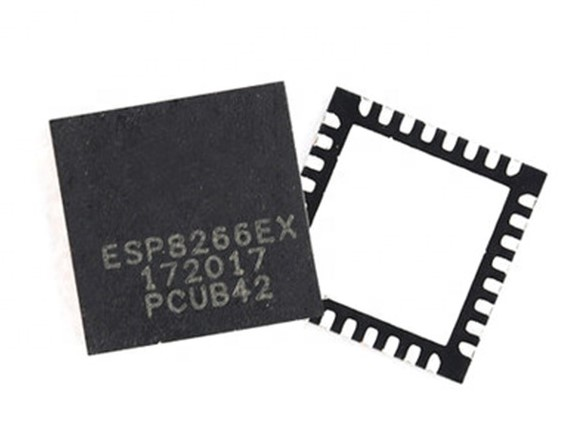
\includegraphics[width=0.3\textwidth]{figuras/esp8266ex.jpg}
        \caption*{\small{DIGIKEY, 2020}}
        \label{fig:esp8266ex}
    \end{figure} 
\end{frame}

\begin{frame}{Elementos de \textit{Hardware}}{O microcontrolador ESP8266}
    \begin{itemize}
        \item Rapidamente se tornou popular como um microcontrolador autônomo devido ao seu baixo custo de mercado;
    \end{itemize}

\end{frame}

\begin{frame}{Fundamentação Teórica}{Elementos de \textit{Firmware}}
\end{frame}

\begin{frame}{Fundamentação Teórica}{Elementos de \textit{Software}}
\end{frame}